\section{Mediciones}

Se realizaron mediciones en base a distintos sets de pruebas que fueron desde 5 elementos hasta 200 elementos. Para cada set, se ejecutó el algoritmo por \textbf{Backtracking}, el algoritmo utilizando \textbf{Programación Lineal}, y por último el algoritmo por \textbf{Greedy}.

\begin{figure}[H]
	\centering
	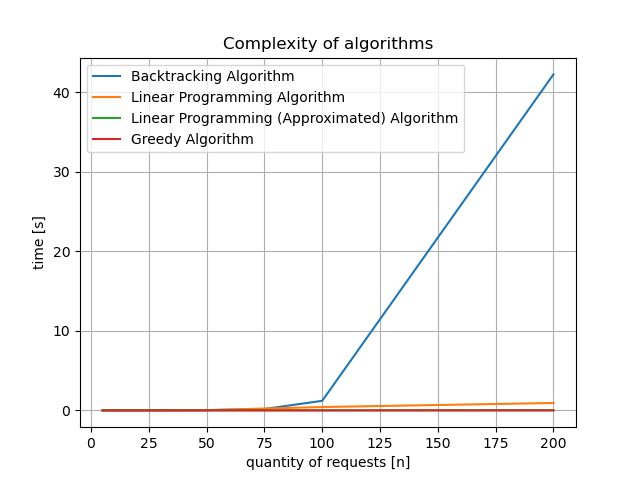
\includegraphics[width=0.9\textwidth]{img/graphic.png}
\end{figure}

Como se puede apreciar, el algoritmo planteado por \textit{Backtracking} es el algoritmo que más tarda con diferencia, haciendo honor a su complejidad respecto a los otros dos. Por detrás de él, está el algoritmo usando la técnica \textit{Greedy}, la cual puede variar su complejidad dependiendo que tan enfocado esté en conseguir el óptimo y en que se base su regla para obtener los óptimos. Esto puede variar tanto su complejidad como qué tan lejos del resultado óptimo se encuentre. Y por último, el algoritmo que más rápido parece haber logrado con diferencia fue el usado con \textit{Programación Lineal}. No solo ha conseguido ser el más rápido, sino que a su vez logró dar la respuesta óptima al problema. Observar que el algoritmo aproximado por \textit{Programacion Lineal} es despreciable en cuanto a lo que tardo, al menos lo que se puede observar en el grafico. Pero los resultados en cuanto a la optimalidad de la solucion difieren cada vez mas en cuanto los subconjuntos son mayores.

Por otro lado, aunque algunos algoritmos sean mas eficientes, pueden ser menos optimos como se puede apreciar:

\begin{figure}[H]
	\centering
	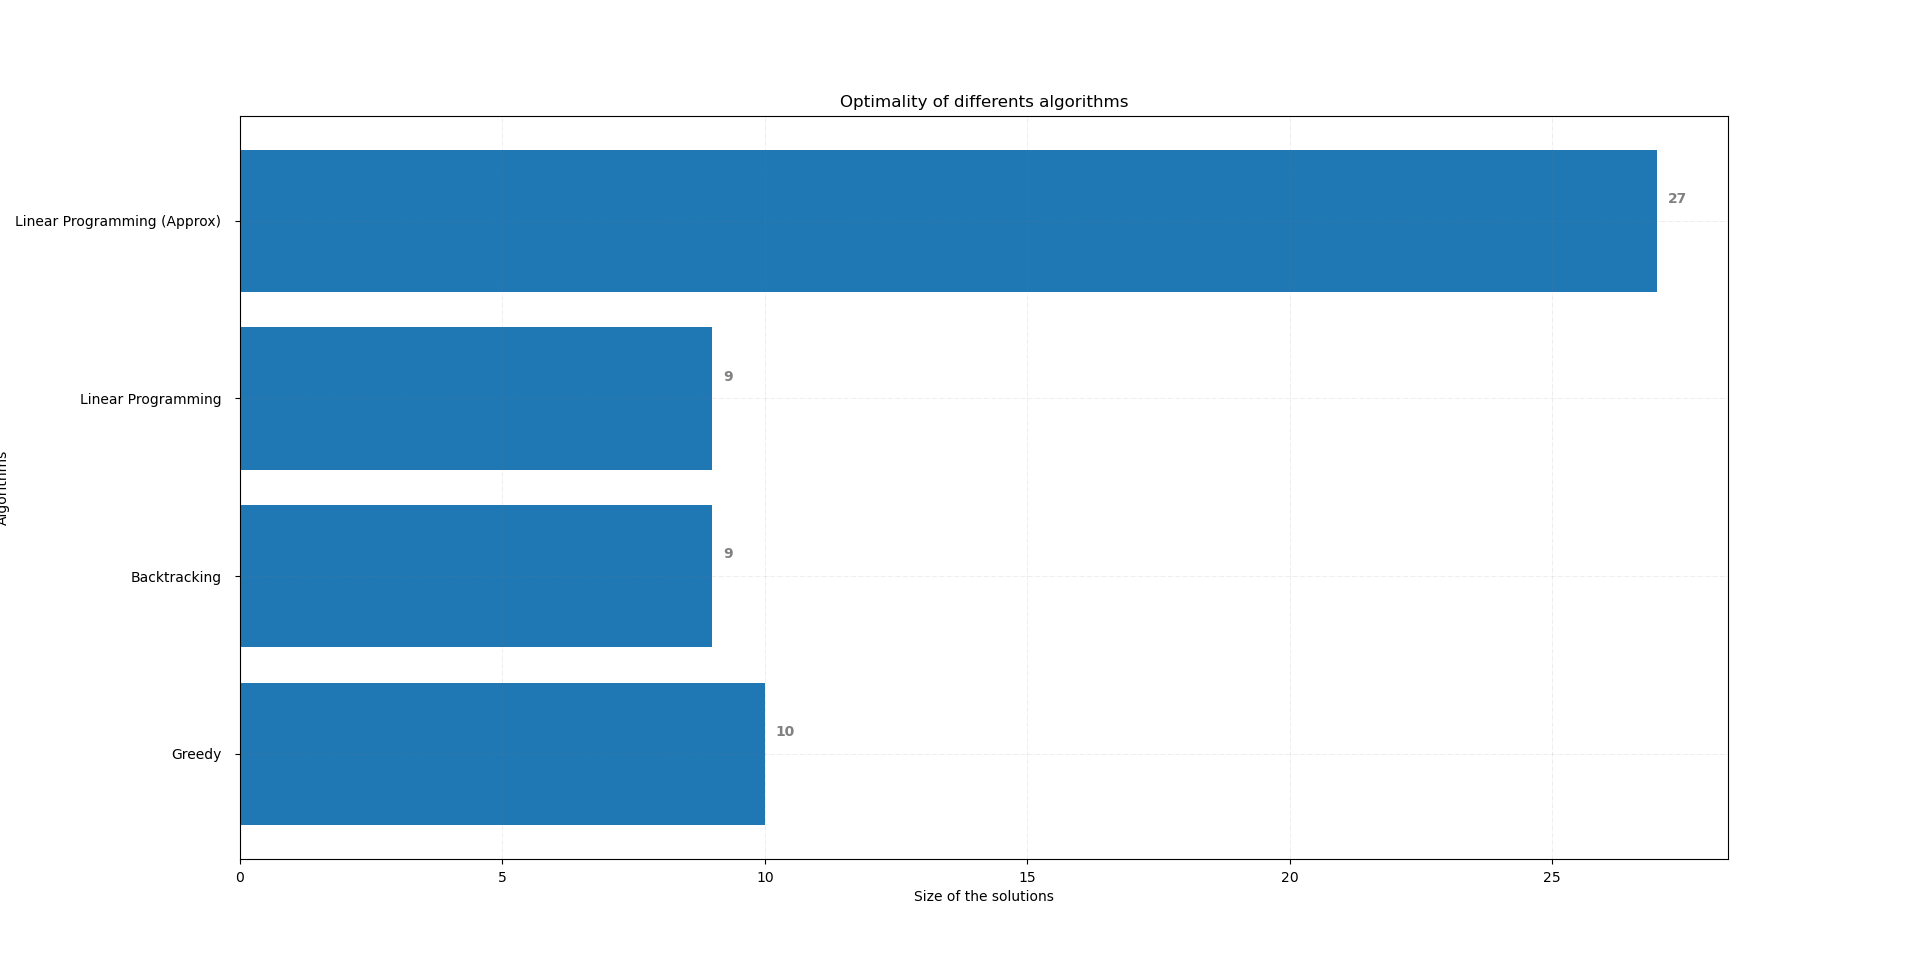
\includegraphics[width=0.9\textwidth]{img/comparison.png}
\end{figure}

Se utilizo un \textit{dataset} de 200 subconjuntos para estas mediciones.

Como podemos observar, el algoritmo por \textit{Backtracking} da siempre la solucion optima (ya que esa es su naturaleza al ver todas las posibles soluciones con sus debidas situaciones de poda). Por otro lado, tenemos el de \textit{Programacion Lineal Aproximada} que aunque sea muy eficiente, difiere demasiado de la solucion optima. Tambien tenemos la solucion \textit{Greedy}, que aunque tambien es eficiente, difiere de la optima aunque con menos distancia de la que se obtuvo con la programacion lineal aproximada. Y por ultima la solucion por \textit{Programacion Lineal} es la que sin duda la mejor opcion para este problema, ya que fue una de las mas eficientes y pudo dar la solucion optima al problema.